\documentclass[12pt, a4paper]{article}
\usepackage{graphicx}
\graphicspath{ {images/} }
\usepackage{amsmath} % many things
\usepackage{physics} % (partial) derivatives, etc.
\usepackage{siunitx}

\let\oldexp\exp
\renewcommand{\exp}[1]{\ensuremath{\oldexp \left( #1 \right)}}
%\renewcommand{\exp}[1]{\ensuremath{\left(#1\right)}}

\textwidth=170mm
\textheight=250mm
\hoffset= -20mm       % may need change
\voffset= -25mm       % may need change

\begin{document}
%% we create our own title page
\thispagestyle{empty}     % only for frontpage
\null\vspace{40mm}
\begin{center}
{%%%%%%%%%%%%%%%%%%%%%%%%%% Title
\Large  Magneto-Optical Trap
\footnote{\noindent Experiment F20, performed on 26\textsuperscript{th} August 2019,
Supervisor Saba Zia Hassan,
short special evaluation}
}\\[15mm]
%%%%%%%%%%%%%%%%%%%%%%%%%%% Authors
L. Hahn and L. Kuehmichel

\vspace{25mm}

\parbox{0.9\textwidth}{
Abstract:    
\small The abstract should preferentially be in English. Here we explain in a
few lines (i) what was done, and (ii) what the results were.
}
\end{center}

\vfill
Audited as a special evaluation: Date, Signature:
\vspace{20mm}

%% Empty backside of title page, remove for single-sided printing
% \newpage  
\null\thispagestyle{empty} 
   
%\newpage
%\tableofcontents 

\newpage

\pagenumbering{arabic} %% start page 1 
\section{Einleitung}
Der XY-Effekt wurde mit der Fisimatenten-Methode gemessen. Dabei $\ldots$ 
war uns nicht immer wohl, da diese Methode zwar genau, aber sehr unpr\"azise 
ist. Das Ziel war die Bestimmung des XY-Koeffizienten. 

N.B. Die \"Uberschriften der Abschnitte sind Vorschl\"age, im Einzelfall 
k\"onnen sie spezifischer, bzw.\ 
die Gliederung auch \"uberhaupt anders sein.

\section{Versuchsanordnung}

Die Versuchsanordnung beruhte auf der XY-Methode. Dabei hatten wir als
Detektor ein gelbes Afo, das geflostert und eriert war \cite{afo} (die Zauberkreide dazu .

Der Text geht weiter, das Bild (ein sog. float) wird irgendwo in der N"ahe des
Aufrufs eingesetzt. Der Abschnitt hier wird in Latex durch 
$\backslash\backslash$ oder $\backslash$par
oder eine Leerzeile erzeugt.

%% die obige Leerzeile macht einen neuen Abschnitt, ebenso \par
%% \\ macht einen Zeilenumbruch, \\[10mm] mit vertikalem Abstand von 10 mm
%
% Wenn Sie den LATEX code durch Leerzeilen strukturieren wollen, dann die Zeile
% 
% mit % beginnen, dann hat sie keinen Einfluss auf das Layout
%
Der Text geht weiter, das Bild (ein sog. float) wird irgendwo in der N"ahe des
Aufrufs eingesetzt, so dass es nicht \"uber die Seitengrenze gebrochen wird.
Der Text geht weiter, das Bild (ein sog. float) wird irgendwo in der N"ahe des
Aufrufs eingesetzt, so dass es nicht \"uber die Seitengrenze gebrochen wird.
Der Text geht weiter, das Bild (ein sog. float) wird irgendwo in der N"ahe des
Aufrufs eingesetzt, so dass es nicht \"uber die Seitengrenze gebrochen wird.
Der Text geht weiter, das Bild (ein sog. float) wird irgendwo in der N"ahe des
Aufrufs eingesetzt, so dass es nicht \"uber die Seitengrenze gebrochen wird.
\begin{figure}[bh]
  \centering
% hier schon der komplixiert Fall, dass 2 Bilder nebeneinander gesetzt werden
  \parbox{60mm}{
    \centering
    %\includegraphics[width=31.5mm]{coord.eps}
%% Dieses Bild ist mit xfig (LINUX) gemacht
    \caption{Coordinate system for 3-D calculations}
  }
  \hfill  % fuegt Platz ein, das rueckt die beiden Bilder an den Rand
  \parbox{60mm}{
    \centering
    %\includegraphics[width=48mm]{coordxy.eps}
    \caption{Coordinate system for 2-D calculations}
  }
\end{figure}
Der Text geht weiter, das Bild (ein sog. float) wird irgendwo in der N"ahe des
Aufrufs eingesetzt, so dass es nicht \"uber die Seitengrenze gebrochen wird.
Der Text geht weiter, das Bild (ein sog. float) wird irgendwo in der N"ahe des
Aufrufs eingesetzt, so dass es nicht \"uber die Seitengrenze gebrochen wird.
Der Text geht weiter, das Bild (ein sog. float) wird irgendwo in der N"ahe des
Aufrufs eingesetzt, so dass es nicht \"uber die Seitengrenze gebrochen wird.
Der Text geht weiter, das Bild (ein sog. float) wird irgendwo in der N"ahe des
Aufrufs eingesetzt, so dass es nicht \"uber die Seitengrenze gebrochen wird.
Der Text geht weiter, das Bild (ein sog. float) wird irgendwo in der N"ahe des
Aufrufs eingesetzt, so dass es nicht \"uber die Seitengrenze gebrochen wird.
 

\renewcommand{\arraystretch}{1.1}  % zieht die Tabelle etwas auseinander
\begin{table}[htb]               
%%  durch das table environment wird die Tabelle wird so geschoben, 
%%  dass sie ganz auf die Seite passt
%%[p] : eigene Seite
%%[h] : moeglichst genau an der Aufrufstelle plazieren
%%[t] : oben an einer Seite
%%[b] : unten auf einer Seite
%%[xyz] : x ODER y ODER z
%%
%% es geht auch ohne \begin{table} ..\end{table} (oder auch {figure}, 
%% dann erscheint die Tabelle genau da, wo sie augefuehrt ist. Das kann 
%% aber mit dem Seitenumbruch schiefgehen.

\begin{center}
\caption{Synopsis of TPC parameters}
\vspace{4mm}
% {|l|l|}: senkrechte Trennlinien, Spalten linksbuendig. Ohne '|' keine Linie
\begin{tabular}{|l|l|}\hline   
Pseudorapidity coverage & $-0.9<\eta<0.9$ for full radial track length\\
                        & $-1.5<\eta<1.5$ for 1/3 radial track length\\
Azimuthal coverage & $2\pi$ \\
Radial position (active volume) & $845<r<2466$ mm \\
Radial size of vessel           & $780<r<2780$ mm  \\
Length (active volume)          & 5000 mm \\
Segmentation in $\phi$		& 18 sectors\\
Segmentation in r		& 2 chambers per sector\\     
Segmentation in z		& central membrane, readout on 2
end wheels \\
Total number of readout chambers & $2\times2\times 18 = 72$ \\ \hline
Inner readout chamber geometry  &  trapezoidal, $ 848<r<1320$ mm active\\
\quad pad size                  & $4\times7.5$ mm\quad ($\phi\times r$)\\
\quad pad rows			& 63 \\
\quad total pads		& 5504 \\ \hline
Outer readout chamber geometry  &  trapezoidal, $ 1346<r<2466$ mm active \\
\quad pad size                  & $6\times10$ and $6\times15$ mm
         \quad ($\phi\times r$)\\
\quad pad rows			& $64+32=96$\quad (small/large pads) \\
\quad total pads		& $4864 + 5120 = 9984$\quad (small/large pads) \\ 
\hline
Front end cards                 & 121 per sector $\times$ 36 = 4356 \\
Readout control unit scheme     & 6 per sector, 18 to 25 FEC per RCU \\
total RCU's                     & 216 \\
Total pads / readout channels   & 557568\\
\hline
Event size \hspace{12mm} for d$N$/d$y = 8000$ & $\sim$60 MB\\
Data rate limit                 & 400 Hz minimum bias\\
Trigger rate limits             & 200 Hz central (limited by space charge)\\
                                & 1000 Hz proton-proton\\ \hline
\end{tabular}
\end{center}
\end{table}

\section{Versuchsdurchf\"uhrung}

Beispiel f\"ur einen Unterabschnitt:

\subsection{Eichung}
Die Flosterung wurde durch Fisimatenten geeicht, das Ergebnis ist in
Abb.~\ref{eichung} gezeigt. 
\begin{figure}[h]
  \centering
  %\includegraphics[height=6cm]{l3-2.eps}
%% Dieses Bild wurde mit PAW erzeugt, nach dem Plotten der Kurven und des 
%% Textes durch den Befehl
%% p/print l3-2.2c.eps 
%% \label{eichnung} bewirkt, dass \ref{eichung} die Bildnummer gibt. Erfordert
%% aber (beim ersten Mal) zwei Durchlaeufe mit latex, die Referenz wird beim 
%% ersten in .aux eingetragen, beim zweiten verwendet.
  \caption{Beispiel f\"ur eingebundenes eps-File (`encapsulated postscript')}
  \label{eichung}          
\end{figure}
Wie man sieht, ist die Eichung gut gelungen; die typischen Abweichungen der 
Eichpunkte von der Eichkurve sind 2.5\%, in \"Ubereinstimmung mit der 
Fehlerrechnung (s.u.).

Weiteres Bla $\cdots$ Bla bla $\ldots$





















\section{Data Analysis}
\subsection{Spectroscopy}
\subsubsection{Multiplet Separation}

%%% LARS ANFANG %%%
During the experiment, all data was recorded in Volts rather than frequency, energy, et cetera. Therefore, to analyse the spectral data of the Rubidium 85 and 87 D2 lines, we first need to calibrate the horizontal axis. In all atoms, energy levels are only observable through absorption or emission of a photon by an electron jumping from one level to another. Due to this, it is not possible to know the absolute energy a level possesses. Only the difference between two levels is observable. As such, we can only infer a cardinal interval scale to the horizontal axis, meaning the zero point is arbitrary.

First, we plotted the full spectrum in which all fine energy level dips are visible. The plot looked as we anticipated, showing 4 separated large (gaussian) dips, accommodated with several smaller peaks near their middle. In order to find the mean value each dip is at, we fitted a gaussian added with a linear background function to each of the profiles:

\begin{equation}
A_0 \exp{\frac{-(x - \mu)^2}{2 \sigma^2}} + ax + b
\end{equation}

Where $A_0$, $\mu$, $\sigma$, $a$, and $b$ were fit parameters, with $A_0$ representing the amplitude, $\mu$ the dip's mean value, $\sigma$ the standard deviation and $a$ and $b$ being background parameters.

\begin{figure}
    \centering
    \parbox{0.45\textwidth}{
        %\centering
        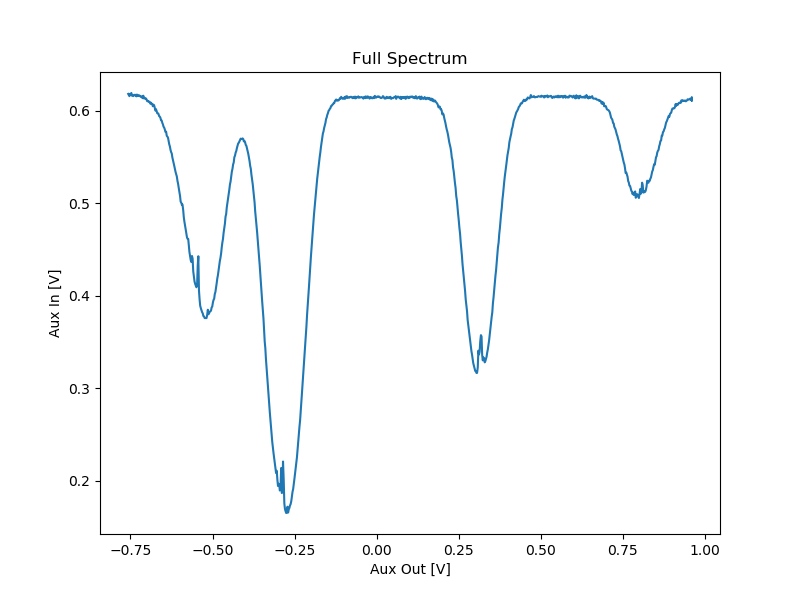
\includegraphics[width=0.5\textwidth]{fullspectrum.png}
    }
    \hfill
    \parbox{0.45\textwidth}{
        %\centering
        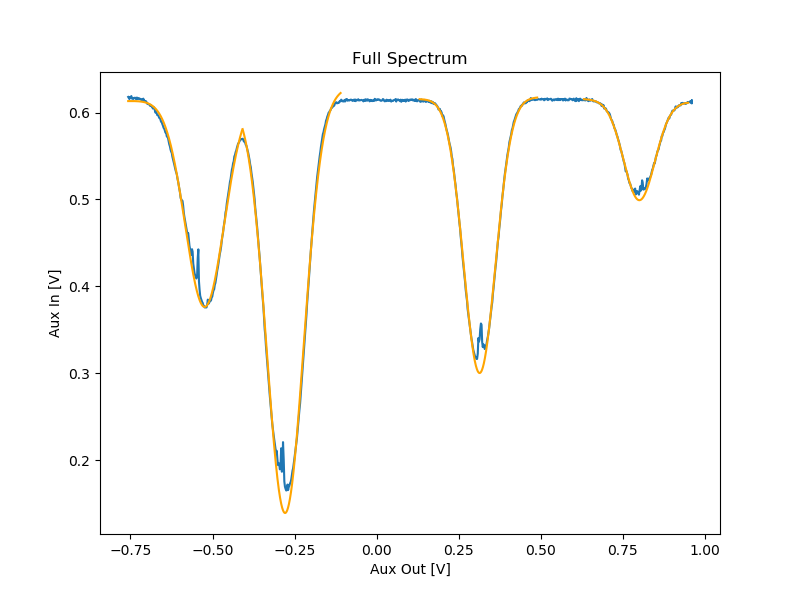
\includegraphics[width=0.5\textwidth]{fullspectrumgaussian}    
    }
    \caption{Left: Full Spectrum. Right: Gaussian Fits}
\end{figure}

Using the separations in $(\mu \pm \sigma)$ from one another, we can derive the calibration from the literature value of these separations. With the literature value\footnote{$= 6.8346826109042(90)\;\si{\giga\hertz}$} for the larger separation between Rubidium 87 $F = 1$ and $F = 2$, we can calculate

\begin{equation}
\dv{V}{f} = (1.9366 \pm 0.0008) \cdot 10^{-10} \quad \si{\frac{\volt}{\hertz}}
\end{equation}

We then use the reciprocal of this value to convert any difference in volts $\Delta V$ to a difference in Hertz $\Delta f$:

\begin{equation}
\Delta f (\Delta V) = \frac{\Delta V}{\dv{V}{f}}
\end{equation}



asdfasfdasdfasdfasdf
























%% Bilder: Sie sollten nicht versuchen, postscript 'from scratch' selbst zu
%% schreiben, sondern den Output von Analyseroutinen (PAW, ROOT, ...) oder
%% von Plot-Programmen (xfig, tgif) verwenden

\begin{figure}[h]
  \centering
  %\includegraphics[width=8cm,bbllx=112,bburx=447,bblly=264,bbury=582]{fig4.ps}
  %\includegraphics[width=8cm]{fig4.eps}  
  \caption{Beispiel f\"ur eingebundenes Postscript-File}
  \label{ps}
\end{figure}

Als erstes machen wir mal eine Gleichung im fortlaufenden Text (sog.\ math mode in LATEX): $s=\frac{1}{2}
a t^2$, dann kommt eine separate gesetzte (sog.\ displaymath in LATEX):
\[         s=\frac{1}{2}a t^2              \]  % die Leerzeichen tun nichts
und dann geht's weiter im Text. Vielleicht eine Gleichung mit fortlaufender 
Nummer:
\begin{equation}
 s(t_1)=s(0) + \int_0^{t_1} v(t)\mbox{d}t 
\end{equation}
Symbole in Formeln werden in einem besonderen, kursiven Font
gesetzt, au\ss er Funktionen (z.B. $\sin\Theta$) und Diffentialzeichen 'd' 
(deswegen die Klimmz\"uge in obiger Formel im LATEX). Wenn man die Symbole im
Text benutzt, z.B. den Weg $s$, dann macht man das auch mit {\em math mode}.
Hervorhebungen in {\em kursiv}, oder {\bf fett}. Es gibt nat\"urlich auch 
andere
Schrifttypen z.B.\ {\sf Sans Serif}.

Hier noch etwas zu Bindestrichen: das - ist ein Binde-Strich f\"ur 
zusammengesetzte Haupt\-w"or\-ter, das -- oder --- ein Gedankenstrich. 

Optionale
Trennungen am Zeilen$\backslash$-ende im LATEX so (siehe z.B.\ das vorige 
`Haupt\-w"or\-ter') im LATEX, falls es zu seltsamen
Trennungen oder Nichttrennungen (oft bei deutschen Umlauten) kommt.

\section{Diskussion}

Hier werden alle wesentlichen Ergebnisse nochmals angefuehrt und diskutiert. 
Bild~\ref{ps} 
% \ref{ps} korrespondiert mit \label{ps}. Das kann man fuer
% Bilder, Tabellen oder Abschnitte [\section, \subsection ...] benutzen und
% muss nicht bei jeder Umstellung neu zaehlen und editieren.
ist ein Beispiel fuer ein eingebundenes .ps (nicht .eps).
Hier muss zus\"atzlich eine sog. {\em bounding box} eingegeben werden, das 
sind die Bildgrenzen in Pixels, hier\\
\centerline{\tt bbllx=112,bburx=447,bblly=264,bbury=582[,clip=1]}
(bounding box lower left x, upper right x, dito y). Die {\it bounding box} 
k\"onnen Sie beim Postscriptviewer gv mit dem Cursor ablesen. {\tt clip=1'}
schneidet Grafik au\ss erhalb der {\it bounding box} ab, andernfalls 
k\"onnen werden auch Bildteile au\ss erhalb wiedergegeben (und \"uberschreiben
ggf. Text etc.).

Am Schluss kann man noch eine allgemeinere Bemerkung zum Versuch machen.


\newpage 
%% hier wird 'von Hand' eine neue Seite erzwungen

%% Literatur)

\begin{thebibliography}{00}   % {00}: max 2-stellige Referenznummer

\bibitem{afo} F. Afo, Nature 15 (1905) 23
\bibitem{uwe} Uwe Ludwig, private Mitteilung
\bibitem{karl} Karl Popper, Phys.~Rev.~Lett.~95 (2001) 25
\bibitem{dipl} K. Winter, Diplomarbeit Heidelberg (1968)
\bibitem{bibel} Genesis 3,4

\end{thebibliography}

\end{document}